\chapter{Methodology}
%%WHAT Is inference3
\label{chap:methodology}

In this section we present a methodology to create a decision model supporting the optimal selection of edge and cloud inference for real-time AI applications.
This methodology consists of a multi-step process and can be seen in figure \ref{fig:Methodology}, which this section will dissect into the individual steps.


\begin{figure}[!htb]
\centering
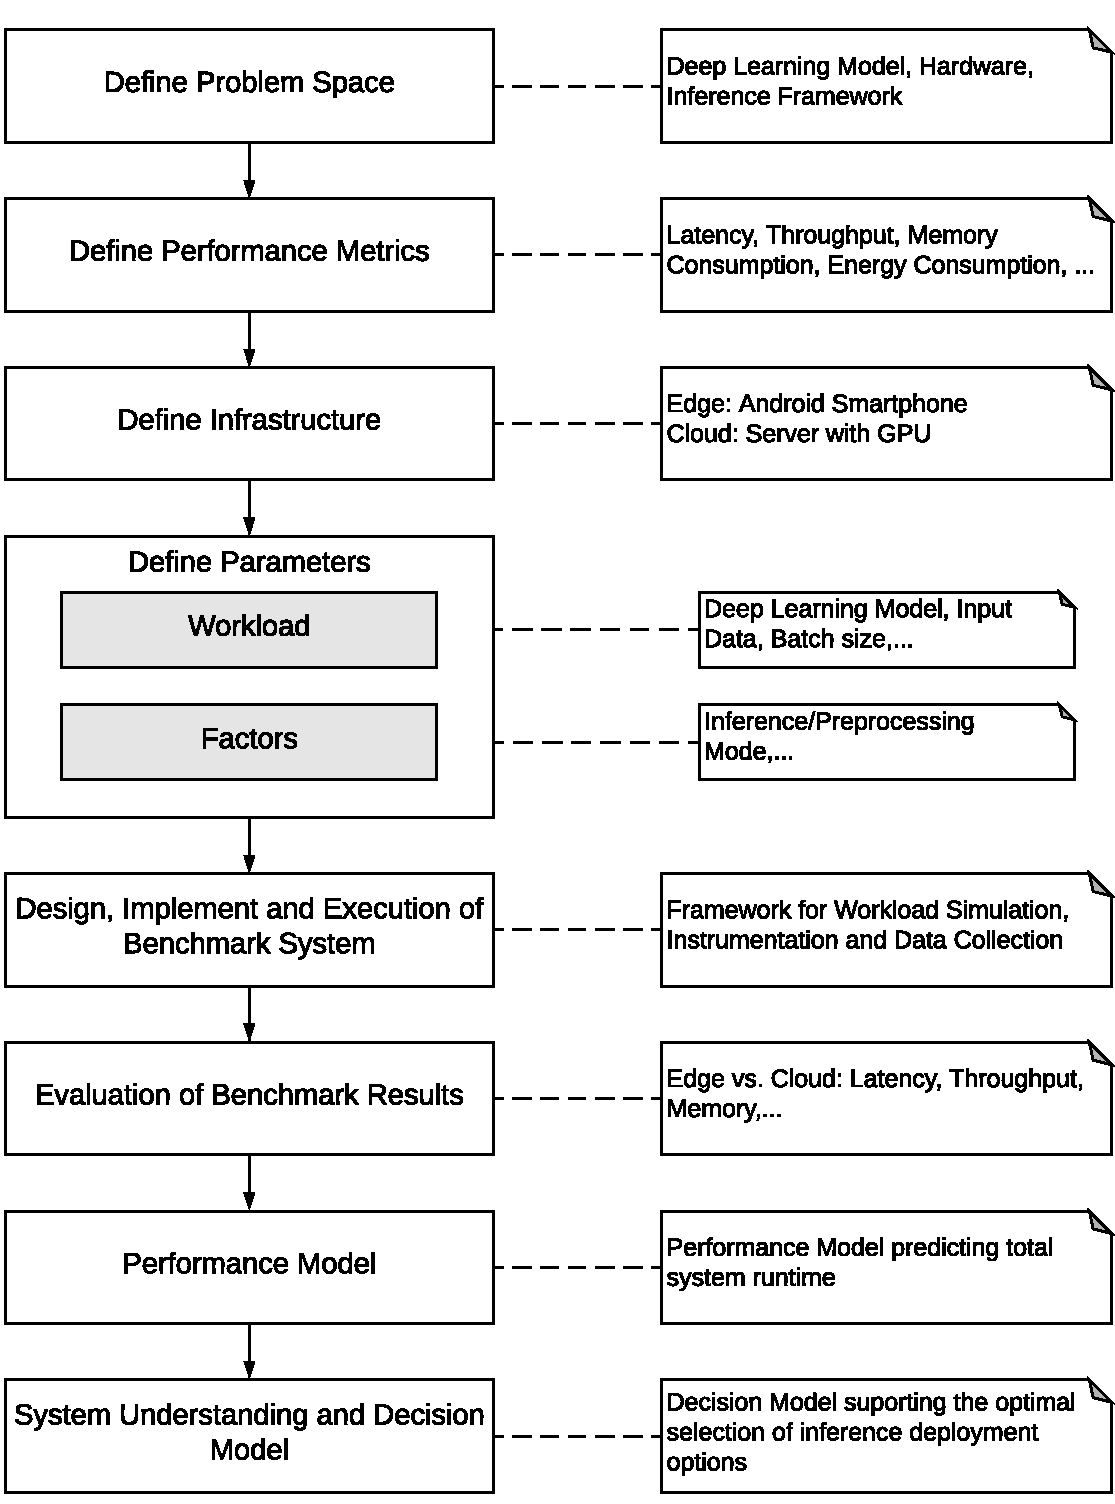
\includegraphics[width=0.96\textwidth]{./Bilder/Methodology.pdf}
\caption{Methodology to help with the optimal selection of cloud and edge inference for real-time AI applications.}
\label{fig:Methodology}
\end{figure}


In order to model the performance of deep learning inference, it is crucial to understand the underlying problem space in a first place.
Therefore all factors influencing the inference performance need to be examined.

Based on the understanding of the problem space the performance metrics then can be derived, which are critical for assessing the inference performance of a deployment option.

The net step is to design an example use case, including real world workload and infrastructure, that is used to illustrate the trade-offs between edge and cloud inference for better system understanding.


After defining the infrastructure, workload and performance metrics a benchmark system can be implemented as a framework for handling workload simulation, performance metrics instrumentation and data collection of the measurements.

Afterwards the collected measurements can be used to evaluate the trade-offs between edge and cloud deployment.
Depending on these trade-offs concrete recommendations can be given for the optimal deployment option in regard to the benchmarked infrastructure and workload.




Using the results of the evaluation and the gained system understanding we then can create a generic decision model for the deployment of deep learning models.
This decision model models the process of deciding whether a deep learning model should be deployed to the edge or to the cloud, not only for the instantiated use case, workload or infrastructure, but as a generic decision model.




%In the next section, we instantiate the presented methodology 



%In order to model the performance of deep learning inference, it is crucial to understand the underlying problem space. 
%In section \ref{chap:fundamentels} we presented the fundamentals of Deep Learning Models, their deployment and the frameworks needed to perform the inference.







\endinput 